\begin{infocard}{Perímetro y área de un triángulo}
Sea $\triangle ABC$ un triángulo rectángulo con lados $a$, $b$ y $c$, como se muestra en la figura \ref{fig:20230402132954}.

\begin{multicols}{2}
    \begin{figure}[H]
        \centering
        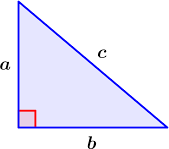
\includegraphics[width=0.9\linewidth]{../images/triangulo_perimetro.png}
        \caption{}
        \label{fig:20230402132954}
    \end{figure}
        El perímetro $P$ es:
        \[P=a+b+c\]
        El área $A$ es:
        \[A=\frac{1}{2}ab\]
\end{multicols}
\end{infocard}